\documentclass{article}
\title{FRG Analysis}
\usepackage{graphicx}
\usepackage{amsmath}
\usepackage{physics}
\usepackage{mathrsfs}
\usepackage{amssymb}
\usepackage{microtype}
\begin{document}
\maketitle
\begin{figure}[!h]
    \centerline{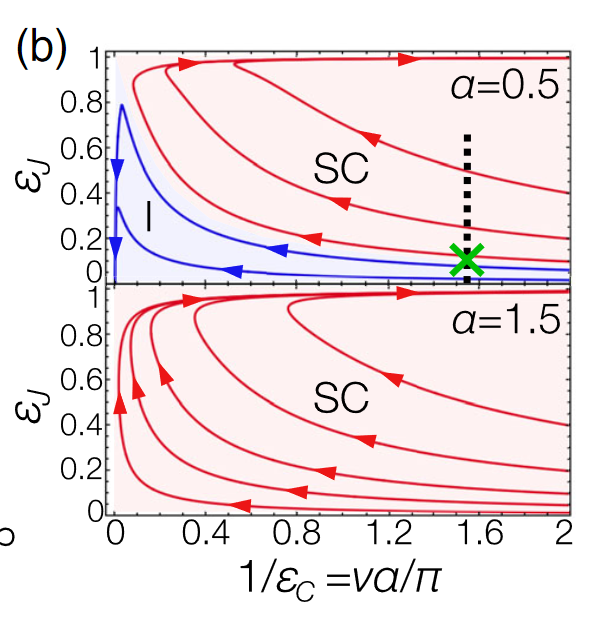
\includegraphics[width=\columnwidth]{Phy129087001_4.png}}
    \caption{Figure.1-(b) Numerical solution of flow equations. $\mu_{10}$ at $\alpha=0.5$}
    \label{figure_1} 
\end{figure}
analysis condition : \\
\textcircled{1} Using functional ansatz, (retaining the most relevant Fourier mode.)\\
\textcircled{2} Renormalized wavefunction.\\
\\
flow equations : \\
 $d_J \ln \epsilon_J = 1- \int^{\infty}_{0}\frac{dy}{\pi}g(y) \dots $ \textcircled{a}\\
 $d_C \ln \epsilon^{-1}_C = -1 + \epsilon^{2}_J\int^{\infty}_{0}\frac{dy}{\pi}h(y) \dots$ \textcircled{b}\\
\\
Equation \textcircled{a} $\rightarrow \epsilon_J \ll 1$ , seperate to two parts,\\
\begin{equation}
    1-\frac{1-\sqrt{2\epsilon_C}{8}} >0 \quad \epsilon^{-1}_C \gg 1
\end{equation}
\begin{equation}
    1-\frac{1}{\alpha} \quad \epsilon^{-1}_C \rightarrow 1
\end{equation}

(2) : \textbf{Presence of DQPT} at $\alpha_C =1$ , previous perturbative result.\\
(1) : \textbf{dangerously irrelevant term $\nu \propto \epsilon_C^{-1}$}.
\\
\\

Because of the dangerously $\nu$,\\
when $\frac{E_J}{E_C}$ is larger than a critical value,\\
Theory flows into the SC fixed point $\alpha < 1$,\\
\textbf{= Absence of DQPT in transmon regimes}

\end{document}